\hypertarget{adat__devel_2lib_2ensem_2ensem__observable_8h}{}\section{/\+Users/archanar/\+Kinematic\+\_\+factor/adat\+\_\+devel/lib/ensem/ensem\+\_\+observable.h File Reference}
\label{adat__devel_2lib_2ensem_2ensem__observable_8h}\index{/Users/archanar/Kinematic\_factor/adat\_devel/lib/ensem/ensem\_observable.h@{/Users/archanar/Kinematic\_factor/adat\_devel/lib/ensem/ensem\_observable.h}}


Observable classes.  


{\ttfamily \#include \char`\"{}ensem\+\_\+obsscalar.\+h\char`\"{}}\newline
{\ttfamily \#include \char`\"{}ensem\+\_\+obsvector.\+h\char`\"{}}\newline
{\ttfamily \#include \char`\"{}ensem\+\_\+obstensor.\+h\char`\"{}}\newline
Include dependency graph for ensem\+\_\+observable.\+h\+:
\nopagebreak
\begin{figure}[H]
\begin{center}
\leavevmode
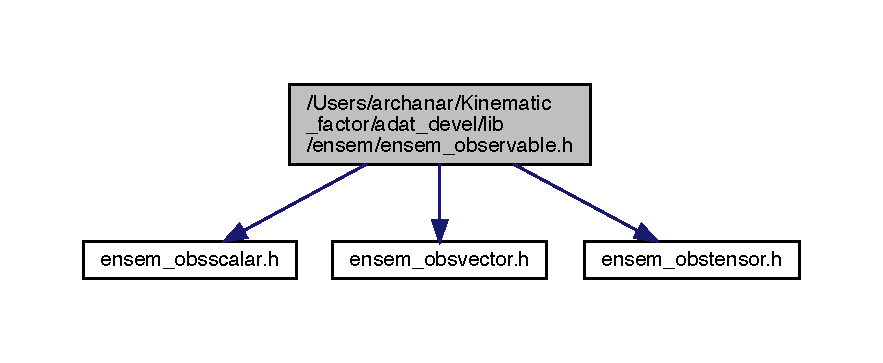
\includegraphics[width=350pt]{da/d91/adat__devel_2lib_2ensem_2ensem__observable_8h__incl}
\end{center}
\end{figure}
This graph shows which files directly or indirectly include this file\+:
\nopagebreak
\begin{figure}[H]
\begin{center}
\leavevmode
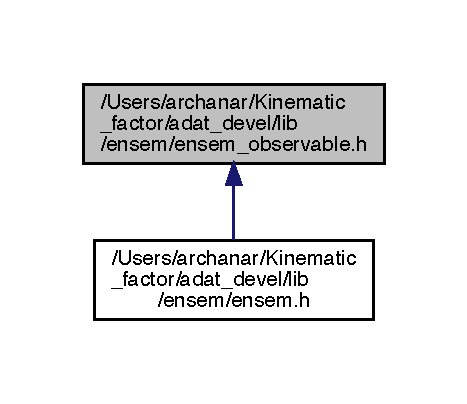
\includegraphics[width=224pt]{d9/da7/adat__devel_2lib_2ensem_2ensem__observable_8h__dep__incl}
\end{center}
\end{figure}


\subsection{Detailed Description}
Observable classes. 

Observables are the various types on the fibers at the lattice sites 